\documentclass{article}
\usepackage[utf8]{inputenc}
\usepackage{tikz}
\usepackage{amsmath}
\usepackage{amsfonts}
\usepackage{amssymb}
\usepackage{fontawesome5}

% TikZ libraries
\usetikzlibrary{shapes, arrows.meta, positioning, shadows, calc}

\begin{document}

\begin{figure}[htbp]
    \centering
    \begin{tikzpicture}[
        node distance=1cm and 1cm,
        block/.style={
            rectangle,
            rounded corners,
            fill=blue!10,
            text width=3cm,
            minimum height=3.5cm,
            align=left,
            font=\small,
            drop shadow
        },
        iconstyle/.style={
            font=\Large\bfseries,
            text=black
        },
        sectiontitle/.style={
            font=\small\bfseries,
            text=black
        },
    ]

    \node (data) [block] {
        \iconstyle{\faDatabase[regular]}
        \sectiontitle{Data}
        \rule{\linewidth}{0.5pt}
        MSTAR \\
        SSDD \\
        HRSID \\
        SARDET
    };

    \node (pre_processing) [block, right=of data] {
        \iconstyle{\faCogs[regular]}
        \sectiontitle{Pre-Processing}
        \rule{\linewidth}{0.5pt}
        SARCNN \\
        NonLocalMeans \\
        MedianFilter
    };

    \end{tikzpicture}
\end{figure}

\end{document}
